\section{Data Design for creative writing evaluation}

\begin{table*}
\def\arraystretch{1.35}
\small
\centering
\begin{tabular}{|l|l|}
\hline
Story                                    & Plot                                                                                                                                                                                                                                                                                                                                                                                                                                                                                                                                   \\ \hline
\href{https://www.newyorker.com/books/flash-fiction/a-triangle}{A Triangle}                               & \begin{tabular}[c]{@{}l@{}}An observer becomes entranced by a seemingly ordinary couple on the street, follows them home,\\ and then watches them from  outside in the rising floodwaters, drawing an eerie connection \\ between the woman and a discarded, burned chair they'd noticed earlier.\end{tabular}                                                                                                                                                                    \\ \hline\hline
\href{https://www.newyorker.com/books/flash-fiction/barbara-detroit-1966}{Barbara,Detroit,1996 }                    & \begin{tabular}[c]{@{}l@{}}On February 12, 1966, a heavily pregnant woman named Barbara experienced a shocking incident in her\\ synagogue in Southfield, Detroit, where a young man shot and killed the renowned Rabbi Adler before\\ turning the gun on himself, and though Barbara tried to reach the shooter, she was swept away by the\\ fleeing crowd.\end{tabular}                                                                              \\ \hline\hline
\href{https://www.newyorker.com/books/flash-fiction/beyond-nature}{Beyond Nature}                           & \begin{tabular}[c]{@{}l@{}}A solitary man walking in a remote mountainous region comes across a car crash, and stays by the side\\ of the lifeless female victim, narrating stories of his past and reflecting on the impermanence of \\events and life itself, while awaiting emergency services amidst the looming presence of wilderness.\end{tabular}                                                                                                                \\ \hline\hline
\href{https://www.newyorker.com/books/flash-fiction/certain-european-movies}{Certain European Movies}                  & \begin{tabular}[c]{@{}l@{}}Two individuals, who are at a residency together, navigate the complexity of their ephemeral relationship \\during their final beach trip, framed by misadventures, subtle tensions, unspoken desires, and \\looming departures.\end{tabular}                                                                                                                                                                                   \\ \hline\hline
\href{https://www.newyorker.com/books/flash-fiction/keys}{Keys}                                     & \begin{tabular}[c]{@{}l@{}}Daniel, struggling with recurring dreams of his ex-wife Rachel and a mysterious unused flat, eventually \\discusses them with his current partner Isabel, sparking various reflections and conversations about their\\ past relationships, until a real-life discovery of old keys triggers a nostalgic memory and helps him find a\\ way to reconnect with his present relationship through canoeing.\end{tabular}                                     \\ \hline\hline
\href{https://www.newyorker.com/books/flash-fiction/listening-for-the-click}{Listening For the Click}                  & \begin{tabular}[c]{@{}l@{}}Navigating a complex social landscape, the protagonist experiences a series of complex relationships \\and emotional turmoil in a student  environment, and engages in self-discovery and self-reflection as she\\ interacts with the characters Carl, Martin, Lizzy, and Johan, resulting in a journey of introspection, betrayal,\\ love, and personal growth.\end{tabular}                                                          \\ \hline\hline
\href{https://www.newyorker.com/magazine/2023/05/15/maintenance-hvidovre-fiction-olga-ravn}{Maintenance, Hvidovre}                   & \begin{tabular}[c]{@{}l@{}}A woman experiences a disorienting night in a maternity ward where she encounters other similarly \\disoriented new mothers, leading to an uncanny mix-up where she leaves the hospital with a baby that she \\realizes is not her own, yet accepts the situation with an inexplicable sense of happiness.\end{tabular}                                                                                                  \\ \hline\hline
\href{https://www.newyorker.com/magazine/2022/11/14/returns}{Returns}                                  & \begin{tabular}[c]{@{}l@{}}The narrator visits their elderly mother in her small town, spending a day with her that is filled with \\nostalgia, conversation, and old habits, only to return a month later after her hospitalization due to\\ a sunstroke, finding remnants of their last visit.\end{tabular}                                                                                                                                                                      \\ \hline\hline
\href{https://www.newyorker.com/books/flash-fiction/the-facade-renovation-thats-going-well}{\begin{tabular}[c]{@{}l@{}}The Facade Renovation That’s \\Going Well\end{tabular}} & \begin{tabular}[c]{@{}l@{}}An academic faculty housed in a building with a critical waterproofing layer missing experiences a series\\ of disruptive and problematic construction repairs, causing tension, inconvenience, and health concerns\\ among the tenants, but ultimately leading to resignation and endurance in hopes of better future\\ circumstances.\end{tabular}                                                        \\ \hline\hline
\href{https://www.newyorker.com/books/flash-fiction/the-kingdom-that-failed}{The Kingdom That Failed}                  & \begin{tabular}[c]{@{}l@{}}The narrator recounts their college friendship with the seemingly flawless Q, and after a decade apart, \\they accidentally cross paths at a pool, where the narrator anonymously observes Q's failed attempt to \\let down a woman about a work-related issue, demonstrating that Q, too, has his share of difficulties.\end{tabular}                                                                                                \\ \hline\hline
\href{https://www.newyorker.com/magazine/2022/06/13/trash }{Trash}                                    & \begin{tabular}[c]{@{}l@{}}A woman unexpectedly marries the son of a successful, ambitious woman named Miss Emily, finding both \\acceptance and critique from her mother-in-law as she navigates this new relationship and confronts the \\stark contrasts between her  former life as a supermarket cashier and her new life as part of a well-off family.\end{tabular}                                                                                                            \\ \hline\hline
\href{https://www.newyorker.com/culture/personal-history/the-last-dance-with-my-dad}{The Last Dance with my Dad}               & \begin{tabular}[c]{@{}l@{}}A young teenager recounts her experiences of fitting into her father's gay lifestyle, highlighted by a\\ seven-day cruise with hundreds of gay men, where she  experienced acceptance and connection, had her\\ first genuine interaction with a  boy, and shared a last dance with her terminally ill father.\end{tabular}                                                                                                       \\ \hline
\end{tabular}
\vspace{2ex}
\caption{\label{teststories} Expert-written short stories from the New Yorker along with their human-verified GPT4 generated summary as plots that are included as part of our test data for Creativity Evaluation}
\end{table*}


Large Language models have been shown to automatically generate long and coherent stories \cite{yang2022doc,yang2022re3} as well as act as collaborators for creative writing \cite{yuan2022wordcraft,ippolito2022creative,mirowski2023cowriting}. However, there have been fewer studies showing how LLM-generated stories differ from expert written stories on metrics that are more fine-grained and objective.Our investigation involves an analysis of a dozen narratives authored by humans, as detailed in Table \ref{teststories}, extracted from The New Yorker. These narratives span a variety of esteemed authors, ranging from \textit{Haruki Murakami} to Nobel laureate \textit{Annie Ernaux}. The protocol for our human assessment incorporates two primary components: 

\begin{itemize}[leftmargin=*]
    \itemsep0em 
    \item Absolute evaluation of creative writing, disregarding whether it has been composed by a human or a LLM
    \item Relative evaluation for discerning whether a story has been produced by a human or an LLM( Turing Test).
\end{itemize}


\begin{figure*}
\centering
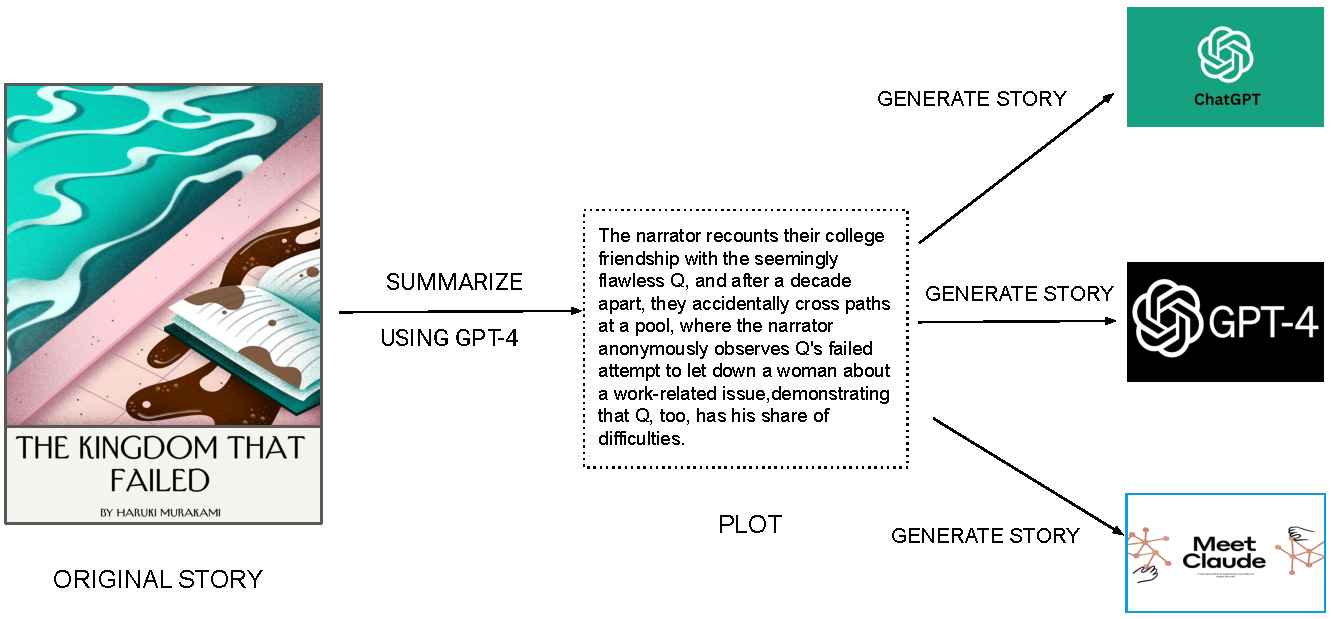
\includegraphics[width=\textwidth]{figures/datapipeline.pdf}
\caption{\label{datapipeline}Pipeline showing how our test set is created for evaluation. For each human-written original NewYorker story, we generate 3 stories from one LLM each, based on the plot of the original story. The plot is a single-sentence summary of the original story automatically generated by GPT-4 and verified by humans.}
\end{figure*}


In order to allow relative evaluation each human-authored narrative is summarized into a single-sentence plot, which is further verified by human evaluators. We then prompt three LLMs: GPT3.5, GPT4, and Claude, to generate a story conditioned on this plot summary. This yields a total of 48 short narratives for absolute evaluation (12 human written; 36 LLM written). Following this, we assign four stories centered around a single plot (one human-authored versus three LLM-authored) to a singular cluster, culminating in a total of 12 clusters. The methodology for creating an individual cluster is illustrated in Figure \ref{datapipeline}. The decision to employ human-authored plot summaries to prompt the LLMs is informed by the recognized shortfall of LLMs in their ability to devise original plotlines, as highlighted in previous research \cite{ippolito2022creative}. Furthermore, the utilization of multiple stories derived from the same plot enables experts to concentrate specifically on the human aspects of creative writing, and enhances their capacity to distinguish human-generated content from AI-produced ones.

In our quest to prevent straightforward parameters from differentiating between stories penned by human authors versus those produced by artificial intelligence (AI), we implemented strategies to ensure comparable story lengths across both classes. Initial experimentation revealed a notable discrepancy: Large Language Models (LLMs), when instructed to generate narratives of a predetermined word count, consistently underperformed, resulting in stories that were invariably more concise than intended. To address this inconsistency, we employed an iterative mechanism, prompting the LLM to iteratively rewrite the initial story until the divergence in word count between the AI-generated and human-composed story was less than 200 for every cluster. Table \ref{promptstory} (Row1) shows the original story prompt, while (Row2) illustrates the subsequent instruction to rewrite the story. We start the iterative process by prompting the LLM to expand the initially generated story. This cycle continued until the narrative length reached the pre-specified threshold or when the iteration count exceeded twenty ($loop\_count > $20). This methodology ensured the creation of AI-written stories with length characteristics more akin to those produced by human authors.

\begin{figure*}
\small
\centering
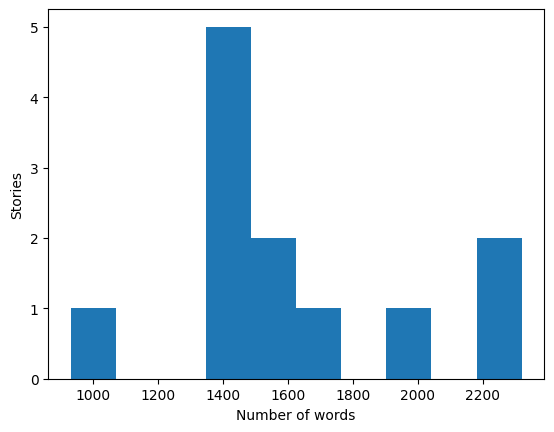
\includegraphics[width=\textwidth]{figures/length.png}
\caption{\label{length} Distribution of word count amongst the stories in our test set}
\end{figure*}


\begin{table}[]
\centering
\small
\def\arraystretch{1.35}
\begin{tabular}{|l|}
\hline
\begin{tabular}[c]{@{}l@{}}Write a New Yorker-style story given the plot below. Make sure it is atleast \textbf{\color{blue}\{\{word\_count\}\}} words. Directly start with the\\ story, do not say things like `Here's the story {[}...{]}:\end{tabular}                                                                                                                                                                                            \\ \hline\hline
\begin{tabular}[c]{@{}l@{}}You wrote the story I gave you below. I requested a story with \textbf{\color{blue}\{\{word\_count\}\}} words, but the story only has\\ \textbf{\color{blue}\{\{current\_word\_count\}\}} words. Can you rewrite the story to make it longer, and closer to the \textbf{\color{blue}\{\{word\_count\}\}} word target\\ I gave you. Directly start with the story, do not say things like `Here's the story {[}...{]}:`\\ \\ Current story: \{\{story\}\}\end{tabular} \\ \hline
\end{tabular}
\vspace{2ex}
\caption{\label{promptstory}Prompt to write the initial story (Row1) vs Prompt to rewrite the initial story to be longer. word\_count represents the number of words in the human written story on a given plot (P) while current\_word\_count represents the number of words in the LLM generated story on the same plot (P)}
\vspace{-7ex}
\end{table}

%     
%     \begin{subfigure}[b]{1.0\textwidth}
%          \centering
%          